\chapter{Il progetto}
\fancyhead[RO]{\bfseries Il progetto}

Dopo aver fatto un'introduzione sulla teoria matematica e sui programmi utilizzati, possiamo ora esaminare il progetto trattato in questa tesi.

L'obiettivo del progetto è quello di offrire un'interfaccia uomo-macchina che permetta all'utente di interagire con la telecamera virtuale presente nella scena utilizzando il proprio volto come controller. Utilizzando la tecnica dell'head-tracking viene rilevato il movimento del volto, che causa la trasformazione della prospettiva con cui è vista la scena, generando l'illusione della presenza di profondità al di là dello schermo. Con un rilevamento efficiente del volto, e con una scena ben fatta, è addirittura possibile creare una visione tridimensionale senza l'uso di occhialini 3D.

Per aumentare l'effetto desiderato, la scena creata inizialmente è l'interno di una scatola, con la parte frontale aperta posizionata sul near plane, in modo da dare l'illusione che lo stesso schermo del pc sia l'apertura della stessa. All'interno si aggiungono degli oggetti per apprezzare meglio i cambiamenti della prospettiva. Ovviamente si possono utilizzare scene di qualsiasi genere ma, per ottenere un effetto maggiore, conviene che i bordi frontali della scena siano fissati ai bordi dello schermo.

L'applicazione è stata sviluppata in due versioni, utilizzando due API differenti: OpenGL e Ogre3D.
Poiché OpenGL opera più a basso livello, le trasformazioni devono essere esplicitate calcolando le matrici e moltiplicandole nel modo opportuno; questo può aiutare nella comprensione delle trasformazioni utilizzate. Tuttavia, dati i miglioramenti che sono stati riportati nella seconda versione, la prenderemo in esame ed analizzeremo il suo codice, trattando le varie fasi in dettaglio.
In seguito sarà dedicata una sezione all'importazione delle scene in Ogre.

L'applicazione è stata scritta in C++ ed è divisa in due parti principali:
\begin{itemize}
\item Un modulo OpenCv separato da tutto il resto, che offre un metodo che fornisce le coordinate del volto rilevate nel momento in cui viene richiamato.
\item La parte grafica sviluppata usando Ogre3D.
\end{itemize}


\section{Il funzionamento dell'applicazione}
Il cuore dell'applicazione risiede nelle trasformazioni da applicare alla scena. In ogni frame vengono eseguite diverse fasi, a partire dall'ottenimento delle coordinate del volto, arrivando a trasformare la telecamera nel modo voluto. In seguito vediamo in breve le fasi:
\begin{enumerate}
\item Ottenimento coordinate del volto in pixel (relative alla webcam).
\item Applicazione di un filtro per eliminare il rumore dato dall'imprecisione del rilevamento.
\item Trasformazione delle coordinate in punti dello spazio 3D.
\item Calcolo dei sei piani del frustum in base alle coordinate dell'osservatore, e creazione della projection matrix.
\item Calcolo dei vettori necessari per la view matrix, e creazione della stessa.
\item Applicazione di una traslazione per aggiustare lo spostamento della telecamera, in modo che la scena sia sempre fissa.
\item La matrice di trasformazione finale relativa alla telecamera è data, in ordine, dal prodotto della matrice di traslazione per la view matrix per la projection matrix.
\end{enumerate}
Analizzando in dettaglio le varie fasi:

\subsection{Coordinate}

Grazie al modulo OpenCv, richiamando una semplice funzione possiamo ottenere le coordinate del volto in un dato frame.\\

Di seguito un estratto di codice della funzione nel modulo OpenCv
\begin{lstlisting}
bool getFaceCoord(int* x, int* y, int* z ) {
...
  if ( detectAndDisplay( pt, z ) ) {
        *x = pt.x;
        *y = pt.y;
        *z = z;
        return true;
    } 
    return false;
}
...

bool detectAndDisplay( cv::Point& center, int& z ) {
...
face_cascade->detectMultiScale( frame_gray, faces, 1.1, 3,
                                0|cv::CASCADE_SCALE_IMAGE, 
                                cv::Size(90,110) );
    
    if (faces.size() == 1 ) { 
            center.x = faces[0].x + faces[0].width*0.5;
            center.y = faces[0].y + faces[0].height*0.1;
            z = faces[0].width;
    }
    return true;
}
\end{lstlisting}
La funzione detectMultiscale rileva i volti e inserisce i risultati in un vettore di matrici, faces.Si controlla che sia rilevato un solo volto, altrimenti si potrebbe generare confusione tra le coordinate.

In seguito sono salvate le tre coordinate:
\begin{itemize}

\item Per la x si considera la coordinata x del centro del volto rilevato.
\item Per la y si considera la coordinata y a $1/10$ dell'altezza del volto, partendo dall'alto. Con varie prove si è notato che gli occhi sono rilevate più o meno a questa altezza, perciò si è adottata questa misura per collegare nel miglior modo la telecamera agli occhi dell'utente.
\item Per la z si considera la larghezza del volto in pixel. Purtroppo non è stato trovato un modo migliore per stimare la distanza dallo schermo, perciò ci si è accontentati di questa misura abbastanza grossolana.  
\end{itemize}


In seguito il codice presente nel parte in Ogre3D, in cui viene richiamata la funzione descritta in precedenza:
\begin{lstlisting}
Ogre::Real x,y,z;
int coordX = 0 ,coordY = 0,coordZ = 0;
if (!getFaceCoord( &coordX, &coordY, &coordZ ) ) {
    x = flX->interpolate(prevX);
    y = flY->interpolate(prevY);
    z = flZ->interpolate(prevZ);
}
\end{lstlisting}
Il metodo getFaceCoord() viene richiamato passando come parametri tre interi. Se la funzione ritorna true si continua con le fasi successive, altrimenti c'è stato un errore nel frame corrente e vengono prese in considerazione le coordinate del frame precedente, per evitare crash nell'applicazione. x, y e z sono di tipo Real, un tipo proprio di Ogre, equivalente al double. Le tre funzioni all'interno del blocco if saranno trattati nella fase successiva.

\subsection{filtro}
Come abbiamo detto nel paragrafo relativo ad OpenCv, vari fattori determinano un riconoscimento non sempre perfetto; ad esempio, rimanendo fermi, le coordinate rilevate oscillano sempre di minimo 2 o 3 pixel, e questo determina una fastidioso tremolio nella scena.

Per ovviare (almeno in parte) a questi problemi, è creato un piccolo algoritmo che filtra il rumore generato dal rilevamento, cercando di preservare la fluidità nei movimenti. In seguito la funzione che elimina il rumore di fondo.
\begin{lstlisting}
void Filter::filter(Ogre::Vector2 &cVec, int erMin,
                                         int erMax) {
    int coord = cVec.x; //coordinata attuale
    int p     = cVec.y; //coordinata precedente
	
    // se coord = 0 il rilevamento non e' avvenuto
    // percio' si considera la coordinata precedente
    if (coord == 0) {
        cVec.x = p;
        return;
    }
    
    int dif = abs( coord - p );
    
    // se e' sotto la soglia minima salva 
    // la coordinata precedente
    if ( dif <= erMin ) {
        cVec.x = p;     	
    }
    // altrimenti pone la precedente uguale all'attuale
    else {
        cVec.y = coord;	
    }  
}
\end{lstlisting} 

La funzione prende in input un vettore con la coordinata attuale e precedente, e una soglia di errore.
Se la differenza in valore assoluto tra le due coordinate è minore della soglia, allora si scarta la nuova coordinata e si utilizza la precedente, non generando movimento nella scena. Questo elimina il rumore, ma genera un altro problema: quando l'utente si sposta normalmente la scena si trasforma con movimenti a scatti, dovuti proprio al filtro che elimina comunque dati utili.

Per risolvere questo secondo problema si è creato un secondo algoritmo che interpola i movimenti, rendendoli più fluidi generando coordinate intermedie tra l'attuale e la precedente. Analizziamo il codice.
\begin{lstlisting}
Ogre::Real FluidFilter::interpolate(Ogre::Real c) {
    // se la coordinata rilevata e' la stessa
    // si avvicina ad essa
    if ( lastCoord == c ) {

        if (count == 1) {
            count--;
            last = c;
        }
        else if ( count > 0) {
            count--;
            last += gap;
        }
    }
    
    // altrimenti ricalcola il gap
    else {
        lastCoord = c;
        count = n;
        gap   =  ( c - last ) / n ;
        last += gap;
    }
    
    return last;
}
\end{lstlisting} 
La classe FluidFilter contiene, fra gli attributi, un contatore e la coordinata interpolata nel frame precedente. Il contatore diminuisce quando le coordinate non cambiano, in modo da rendere l'interpolazione finita. Se le coordinate cambiano invece si calcola un gap dato dalla differenza tra quella attuale e quella interpolata precedentemente, diviso per n; n influisce sulla qualità dell'interpolazione: all'aumento di n i movimenti sono più fluidi, ma, come effetto contrario, sono più rallentati. Con un valore di n pari a 3 o 4 l'effetto finale è accettabile, rendendo il delay quasi impercettibile e la fluidità efficiente.

\subsection{3d}
Le coordinate fornite da OpenCv sono interi che rappresentano il centro del volto rilevato.
Per esempio in una webcam con risoluzione $640\times 480$ la x oscilla tra $0$ e $640$ e la y tra $0$ e $480$; inoltre l'origine si trova nell'angolo in alto a sinistra.

Il sistema di coordinate del mondo 3D è differente ed ha origine nel punto $(0,0,0)$. Perciò le coordinate devono essere trasformate per essere utilizzate nel nuovo sistema di coordinate

Per una maggiore efficienza, le coordinate dovrebbero essere calcolate anche in funzione della distanza dalla telecamera; inoltre dovrebbero variare anche in base alle dimensioni della scena importata. Per ora questo studio non è stato effettuato perciò, utilizzando una scena di default, sono stati adottati i seguenti calcoli:
\begin{lstlisting}
    z = z / 150.0f;
    x = -( ( ( x - xCam/2 ) / 15.0f ) / (xr*ar) );
    y = -( ( ( y - yCam/2 ) / 15.0f ) / (yr*ar) );  
\end{lstlisting}  
\textit{xCam} e \textit{yCam} rappresentano le dimensioni della webcam in pixel. La prima sottrazione nella x e nella y spostano l'origine di OpenCv nell'orgine del mondo virtuale.

\textit{ar} è il reciproco dell'aspect ratio della finestra aperta.

\textit{xr} e \textit{yr} sono rispettivamente il rapporto delle dimensioni della finestra per quelle della webcam, sempre in pixel. Questa divisione finale dovrebbe permettere di mantenere una proporzionalità dei movimenti utilizzando risoluzioni diverse.

\subsection{perspective matrix}
Si calcolano i 6 piani del frustum in base alle coordinate rilevate, in modo da modificare la prospettiva in ogni frame.
\begin{lstlisting}
    n = -face.z + nP;     //near plane
    f = n + sceneLength;  //far plane
    r = width - face.x;   //right plane
    l = r - 2*width;      //left plane
    t = height - face.y;  //top plane
    b = t - 2*height;     //bottom plane

\end{lstlisting}
Il vettore \textit{face} contiene le coordinate calcolate.

Il near plane è calcolato in base alla distanza (approssimata) dell'osservatore, in modo che, quando si avvicina allo schermo, si produce un effetto di allungamento della scena . Per fare un esempio immaginiamo di vedere una finestra da lontano; più ci avviciniamo alla finestra e più ampia diventa la vista di ciò che c'è al di fuori. Inoltre esso varia in base alla costante \texttt{nP} definita dall'utente, che permette di modificare la distanza focale di default a piacimento.

Il far plane dipende dal near plane e dalla lunghezza della scena.

I successivi quattro piani sono calcolati in modo che formino sempre un rettangolo di dimensioni variabili, con lo scopo di ottenere un frustum asimmetrico che distorce la prospettiva della visuale.
\textit{width} e \textit{height} coincidono rispettivamente con la metà della larghezza e dell'altezza della scena. Come vedremo in seguito, queste dimensioni dovrebbero rispettare l'aspect ratio della finestra aperta.

In seguito viene richiamata una funzione che prende in input le sei coordinate e, nello stesso modo che abbiamo visto nella teoria, calcola la matrice di proiezione, restituendola:

\begin{lstlisting}
Ogre::Matrix4 frustum = Ogre::Matrix4(
        
        2*n/(r-l),         0, (l+r)/(r-l),           0,
                0, 2*n/(t-b), (t+b)/(t-b),           0,
                0,         0,     f/(n-f), (n*f)/(n-f),
                0,         0,          -1,           0
);

\end{lstlisting}

\subsection{view}
Come abbiamo visto nel paragrafo relativo alla view matrix, occorrono tre vettori per costruire quest'ultima.
In seguito il codice relativo al calcolo dei primi due vettori:
\begin{lstlisting}

eye    = Ogre::Vector3(-face.x, -face.y, -face.z);

target = Ogre::Vector3(r - width, t - height, -n);
\end{lstlisting}
\textit{eye} utilizza le coordinate del volto, con il segno opposto. Quando il frustum viene spostato lungo una direzione, l'effetto prodotto è uno spostamento della scena nel verso opposto. Questo perchè il frustum rappresenta la porzione di spazio da visualizzare, non la scena. Ad esempio se noi stiamo guardando un oggetto nel frattempo che ci stiamo muovendo verso destra, dal nostro punto di vista l'oggetto si starà spostando verso sinistra. Perciò, per mantenere allineati i movimenti, il vettore \textit{eye} deve essere l'inverso di \textit{face}.
Senza questa accortezza si crea un effetto di rotazione, come è possibile vedere nella figura \ref{wrong-eye}.

\begin{figure}[htbp]
\centering
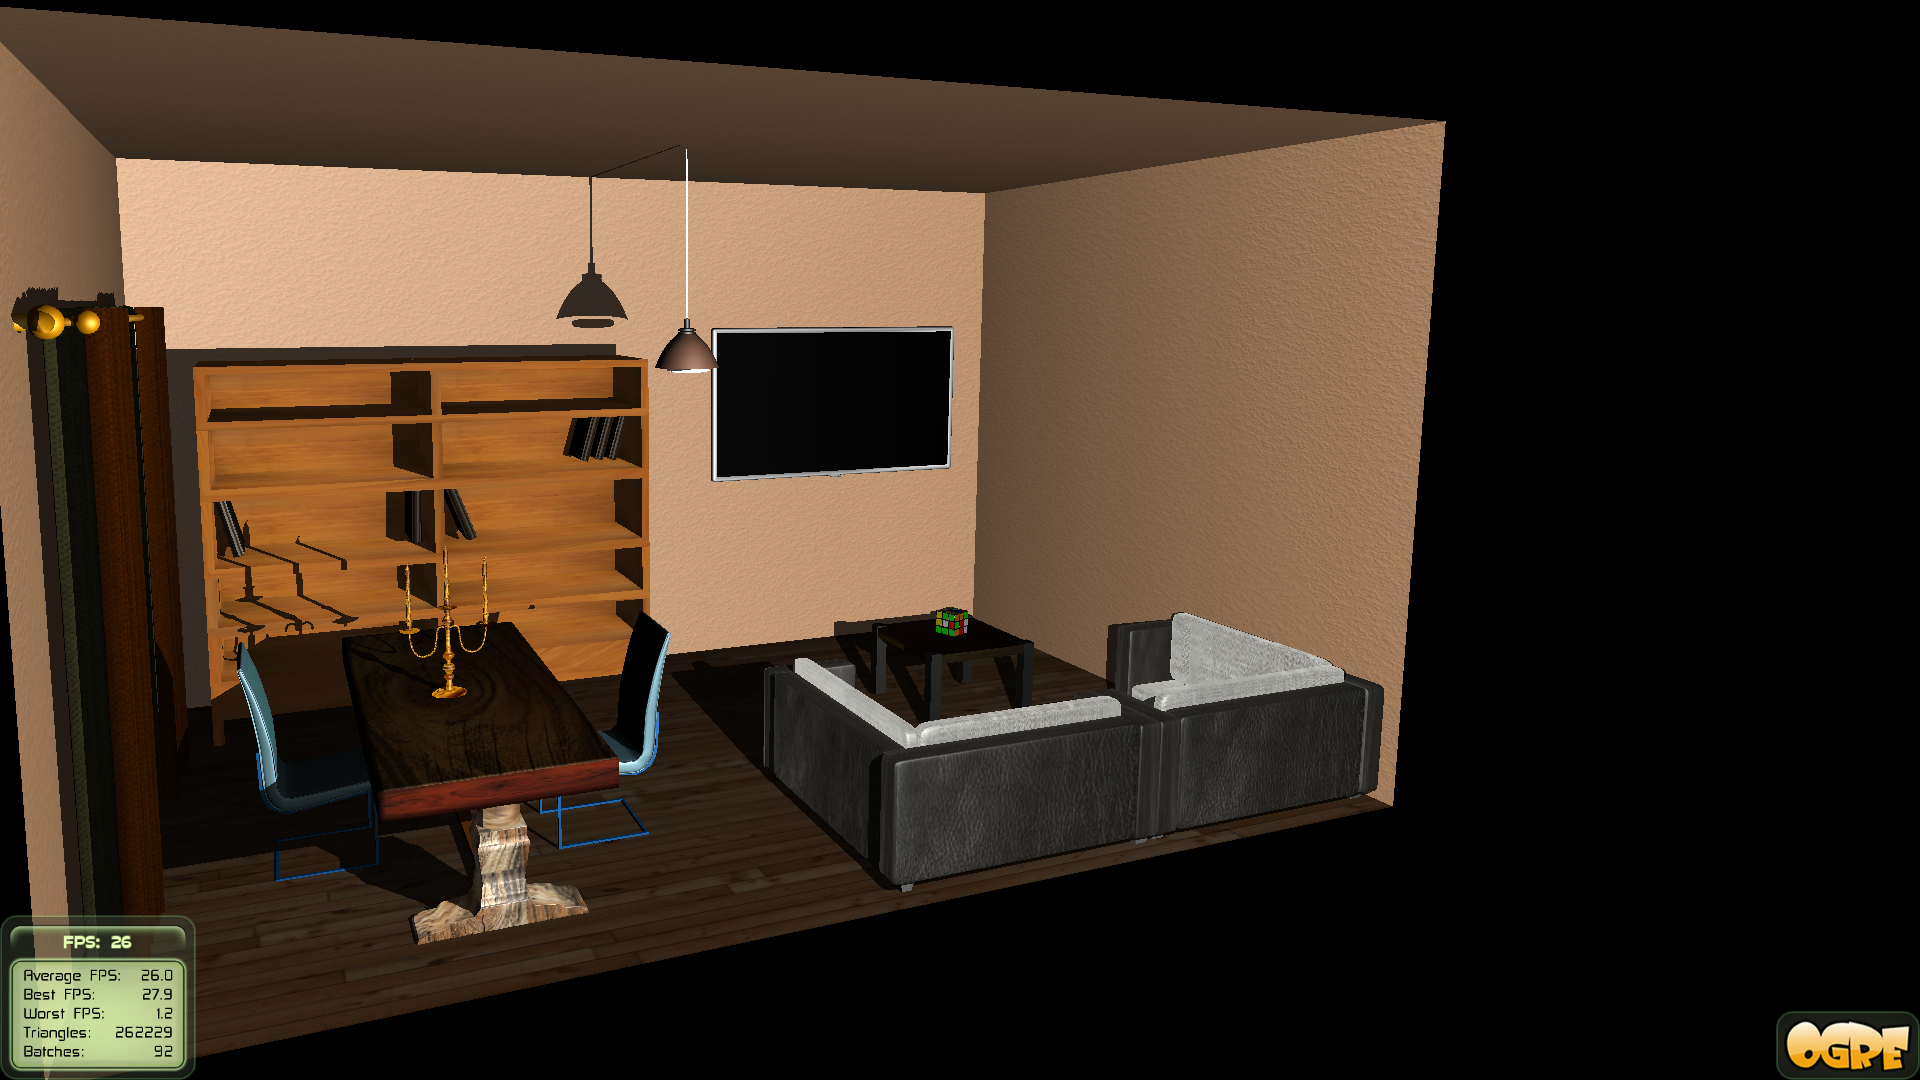
\includegraphics[width=0.7\textwidth]{images/progetto/ogre-wrong.png}
\caption{Trasformazione ottenuta calcolando in modo errato il vettore \textit{eye}.\label{wrong-eye}}
\end{figure}


\textit{target} è il centro del rettangolo che rappresenta il near plane, in quanto il punto osservato deve essere sempre il centro della scena.

In seguito viene richiamato un metodo che calcola la view matrix:
\begin{lstlisting}
Ogre::Vector3 up = Ogre::Vector3(0, 1, 0);
Ogre::Vector3 z = (eye - target); 
z.normalise();     // forward vector.
Ogre::Vector3 x = (up.crossProduct(z)); 
x.normalise();    // right vector.
Ogre::Vector3 y = z.crossProduct(x); // up vector.
 
Ogre::Matrix4 viewMatrix = Ogre::Matrix4(
    x.x, x.y, x.z, -(x.dotProduct(eye)),
    y.x, y.y, y.z, -(y.dotProduct(eye)),
    z.x, z.y, z.z, -(z.dotProduct(eye)),
      0,   0,   0,                    1
);
\end{lstlisting}
Il vettore \textit{up} equivale all'asse Y; la base ortonormale la matrice sono calcolati come è stato visto nella parte teorica.


\subsection{trasl} 
Con le trasformazioni calcolate in precedenza otteniamo colleghiamo la prospettiva della visuale con la posizione dell'utente, però vengono generati anche degli spostamenti indesiderati della scena che la fanno scomparire oltre lo schermo, in quanto la telecamera virtuale in realtà sta fluttuando in base ai nostri movimenti.

Vediamo nella figura \ref{no-transl} l'effetto indesiderato.

\begin{figure}[htbp]
\centering
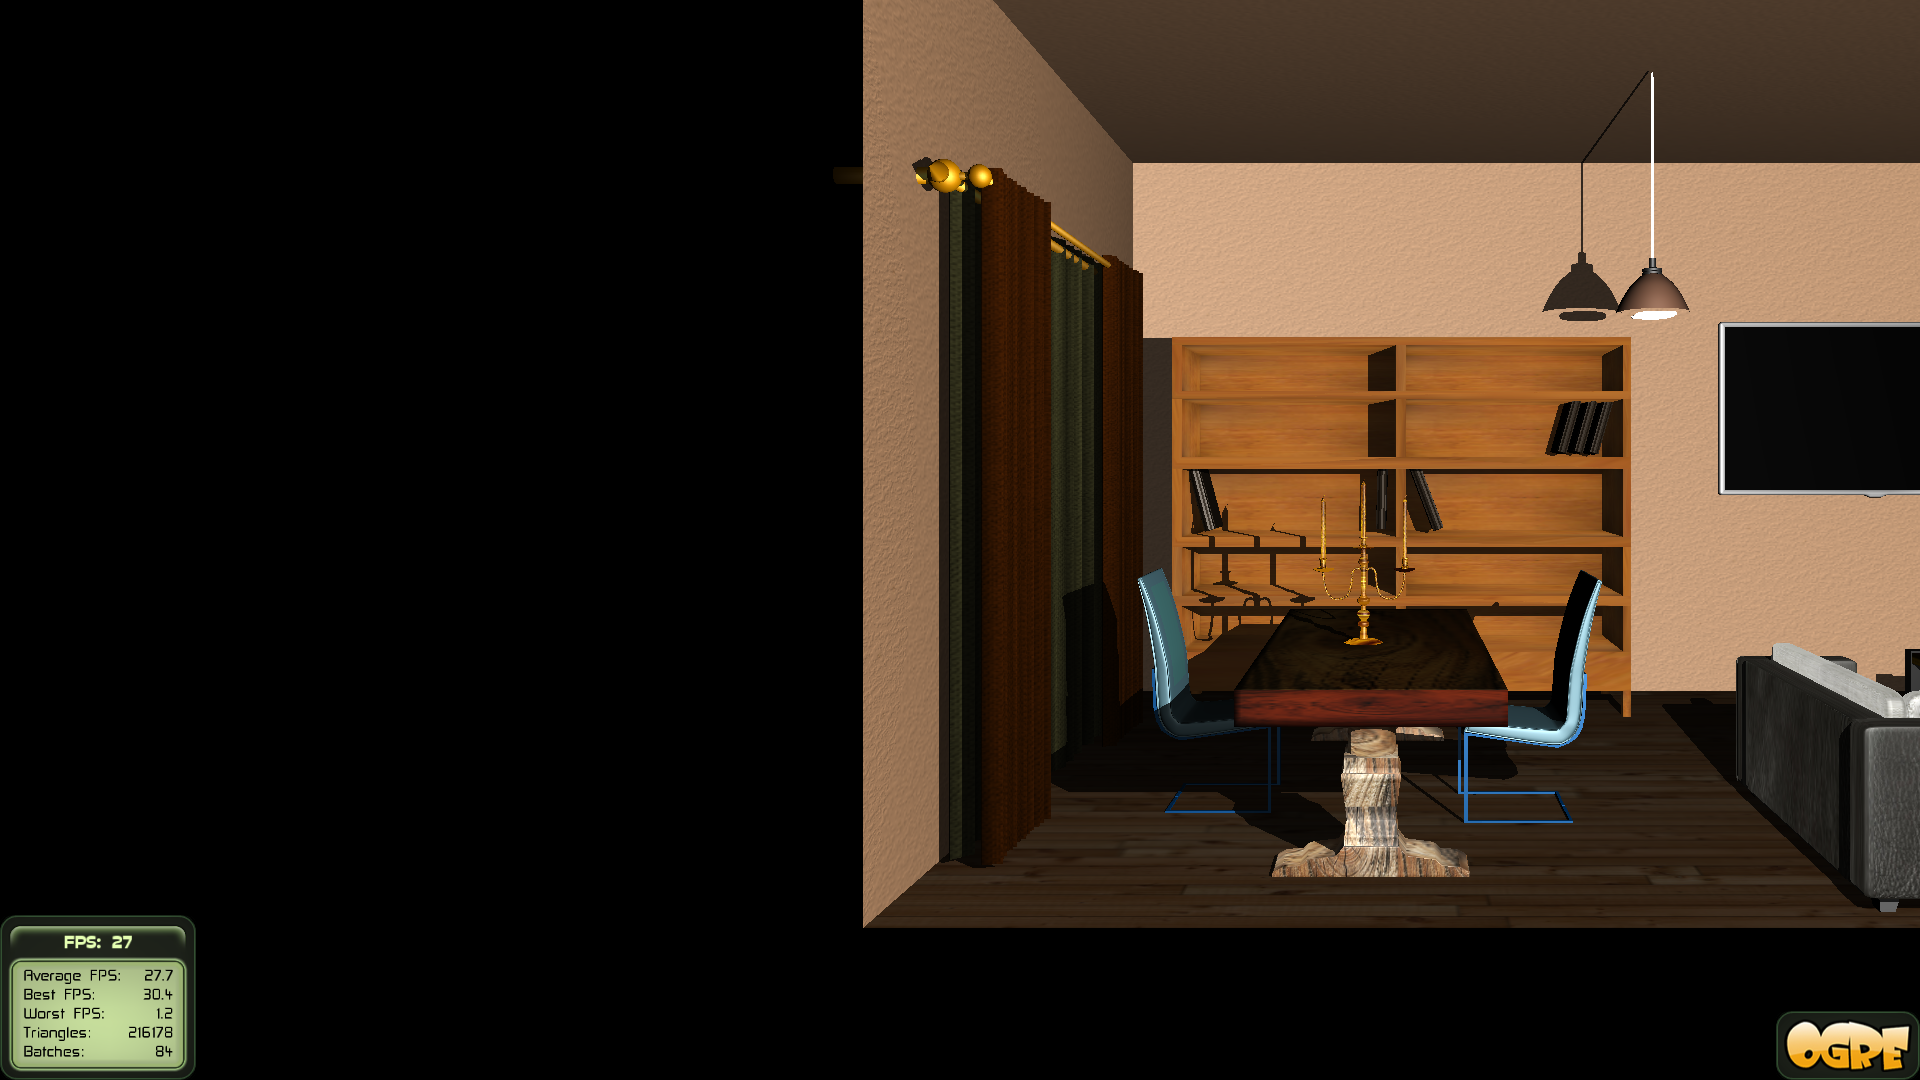
\includegraphics[width=0.7\textwidth]{images/progetto/ogre-transl.png}
\caption{Scena fluttuante, dovuta all'assenza di traslazione.\label{no-transl}}
\end{figure}

La vera forza della trasformazione sta nel fatto che la scena deve invece rimanere ferma, fissata ai bordi dello schermo, e per questo occorre una traslazione che annulli gli spostamenti precedenti.



\begin{lstlisting}
Ogre::Vector3 translVec = Ogre::Vector3(
            -face.x + r - width,
            -face.y + t - height,
            0
    );

Ogre::Matrix4 translMat = Ogre::Matrix4::IDENTITY;
translMat.makeTrans(translVec);
\end{lstlisting}
La matrice di traslazione è calcolata con la funzione \textit{makeTrans}, che prende come parametro il vettore che annulla lo spostamento della telecamera.

\subsection{fine}
In OpenGl la trasformazione della telecamera è rappresentata da una matrice, che è il prodotto tra la traslazione, la matrice di proiezione e la view matrix:
\begin{lstlisting}
camera = translMat * frustum * viewMatrix;
\end{lstlisting}
In Ogre questa operazione è eseguita automaticamente dal framework, quindi basta solamente impostare le due matrici, utilizzando come view matrix il prodotto tra la matrice di traslazione per la view matrix calcolata a mano.
\begin{lstlisting}
mCamera->setCustomViewMatrix(true, translMat*view);
mCamera->setCustomProjectionMatrix(true,frustum);
\end{lstlisting}



\section{Importazione scene in OpenGL}
Un'ulteriore feature che si voleva aggiungere all'applicazione era quella di poter caricare una qualsiasi scena, modellata con programmi come Blender, e poterla visualizzare in modo più interattivo, creando l'illusione 3D.

In OpenGL è utilizzato un parser di file con estensione .obj, in modo da caricarli nel buffer e renderizzarli a schermo. All'avvio del programma viene esaminata una directory apposita e, per ogni file .obj trovato, ne viene fatto il parsing e vengono inserite caratteristiche quali coordinate dei vertici, coordinate uv per il mapping delle texture, etc in diversi buffer.

Purtroppo questo processo si è rivelato oneroso in OpenGl e ha portato anche ad alcune problematiche che hanno determinato la scelta di compiere questo ulteriore passo utilizzando il framework Ogre3D.

\section{Importazione in Ogre3D}
Esistono diversi exporter per software di modellazione quali Blender, Maya, 3D Studio Max, etc, per esportare scene e convertirle nel formato riconosciuto da Ogre. I modelli hanno estensione .mesh, mentre le informazioni relative ai materiali sono raccolte in file con estensione .material, tramite un linguaggio proprio di Ogre, facilmente comprensibile.

Per ottenere effetti più apprezzabili nelle trasformazioni, conviene che la scena rappresentata sia racchiusa da un box, con l'apertura frontale. Come esempio è stata preparata una scena in Blender, raffigurante un salotto, come si può vedere nella figura \ref{liv-room}.

\begin{figure}[htbp]
\centering
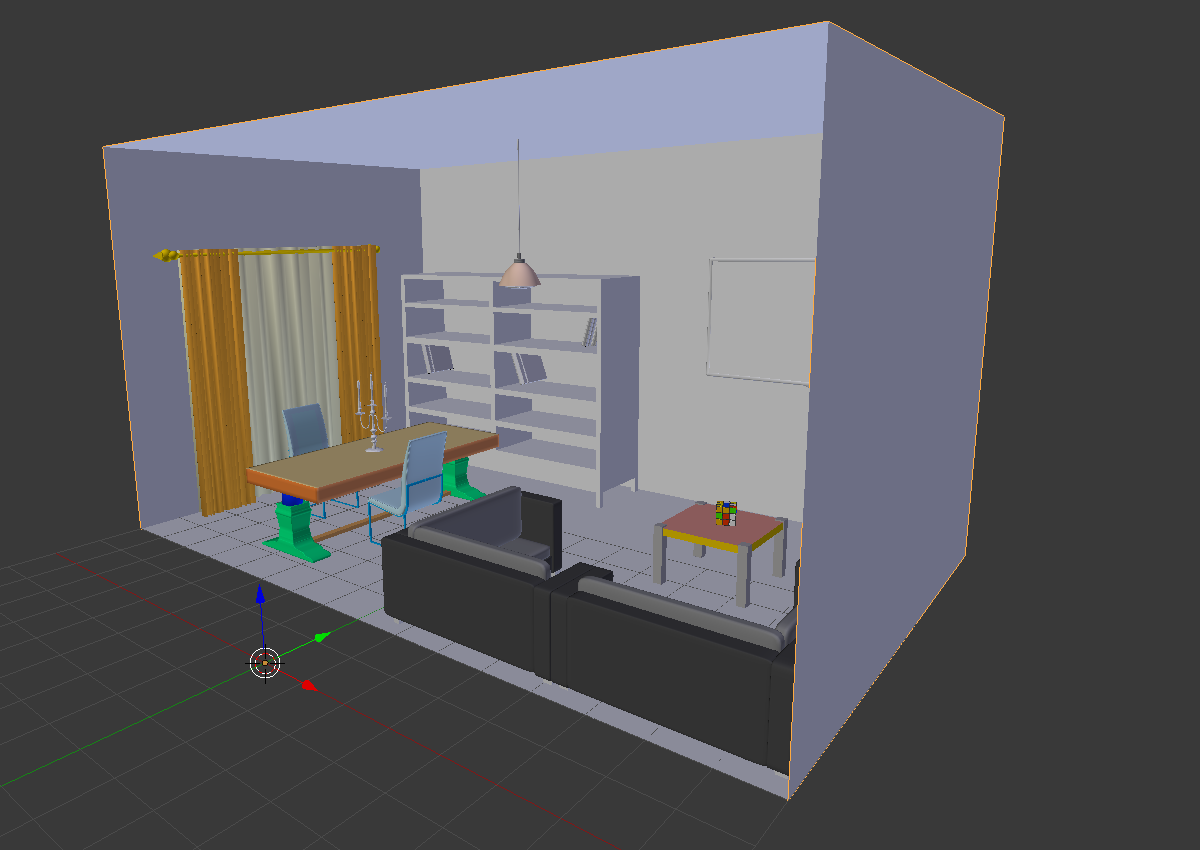
\includegraphics[width=0.7\textwidth]{images/progetto/living-room.png}
\caption{Scena modellata in Blender.\label{liv-room}}
\end{figure}

Da notare il fatto che le misure del box che racchiude la scena, in questo caso, ha un aspect ratio di $16/9$, infatti la lunghezza è pari a 16 unità mentre l'altezza è di 9 unità. Questo perchè lo schermo utilizzato ha lo stesso aspect ratio. In Ogre è possibile scegliere la risoluzione della finestra all'avvio dell'applicazione, perciò si deve fare attenzione a rispettare il formato, in quanto rapporti diversi possono creare effetti di stretching o di rimpicciolimento lungo una o entrambe le dimensioni.

Per ottenere una trasformazione corretta, il nostro frustum dovrebbe avere le stesse dimensioni della scena importata, ed inoltre il near plane va posizionato ad una distanza pari alla distanza da dove comincia la scena, in modo che il near plane coincida con l'apertura del box.

Un'ulteriore operazione da fare, all'avvio dell'applicazione, è quella di traslare la scena in modo che sia centrata nell'origine, per rientrare nella porzione di spazio considerato nel frustum.
Dopo la traslazione la scena sarà posta come è visibile nella figura \ref{transl-liv-room}. L'origine è rappresentato dai tre assi cartesiani colorati.

\begin{figure}[htbp]
\centering
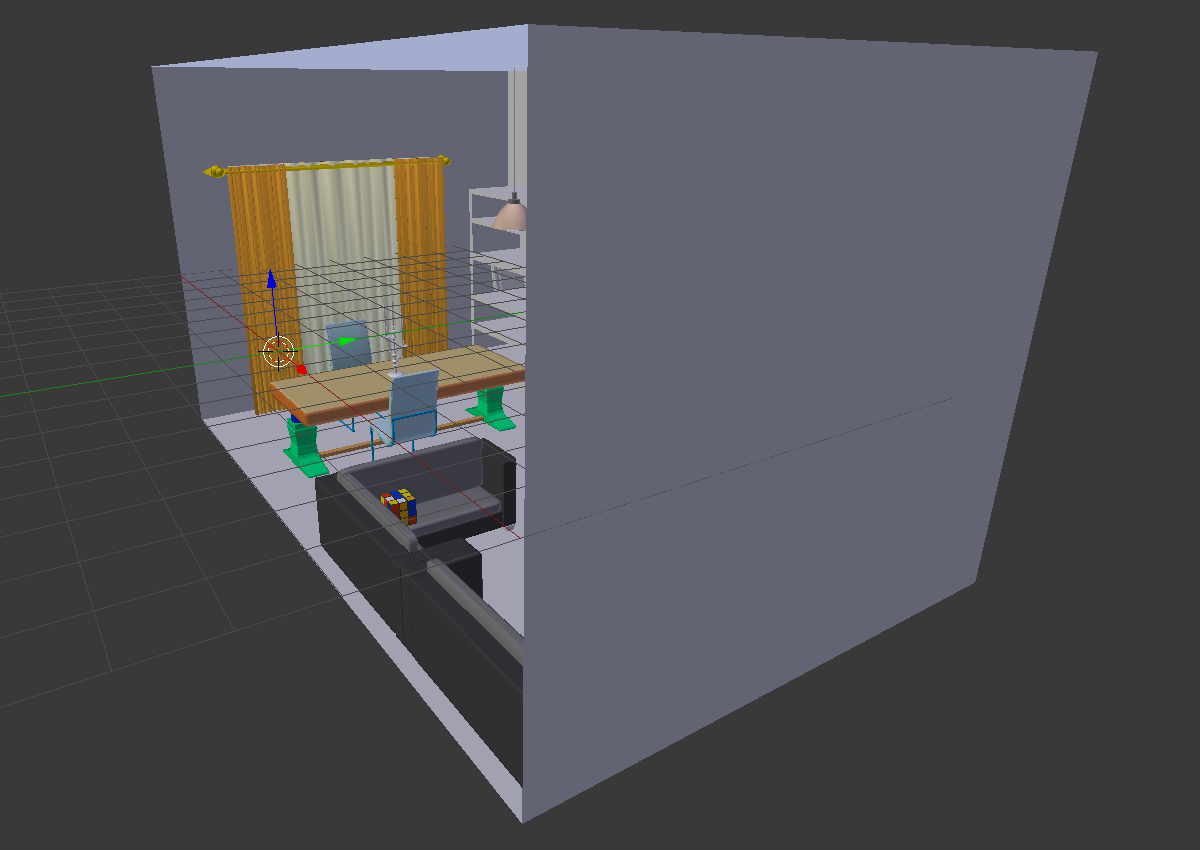
\includegraphics[width=0.7\textwidth]{images/progetto/living-room-translated.png}
\caption{La scena dopo la traslazione.\label{transl-liv-room}}
\end{figure}


Per quanto riguarda la Z,la nostra scena inizia alla coordinata $y=2$ ( la coordinata Y di Blender corrisponde alla Z in Ogre3D), perciò il near plane sarà posto ad una distanza pari a 2 lungo l'asse z, rispetto all'origine. Ovviamente il near plane è variabile, per determinare gli effetti di allontanamento o avvicinamento, ma comunque lo spostamento è corretto dalla view matrix, così che il near plane è sempre coincidente con l'apertura del box.

Tutte queste condizioni sono necessarie affinchè i bordi della scena siano sempre fissati ai bordi dello schermo del pc, in modo da illudere maggiormente l'occhio. Ovviamente senza questi accorgimenti la trasformazione continuerebbe comunque a funzionare in modo corretto, ma gli effetti ottenuti non garantirebbero l'illusione che l'applicazione ha lo scopo di creare.
 

